\subsection{Torseur des efforts résultant}

\begin{frame}
    \frametitle{Torseur des efforts résultants}
    On se place sur un élément de la surface latérale $\partial S \times ]-h_s,h_f[$, de largeur infinitésimale $dl$ :
    \begin{figure}
        \centering
        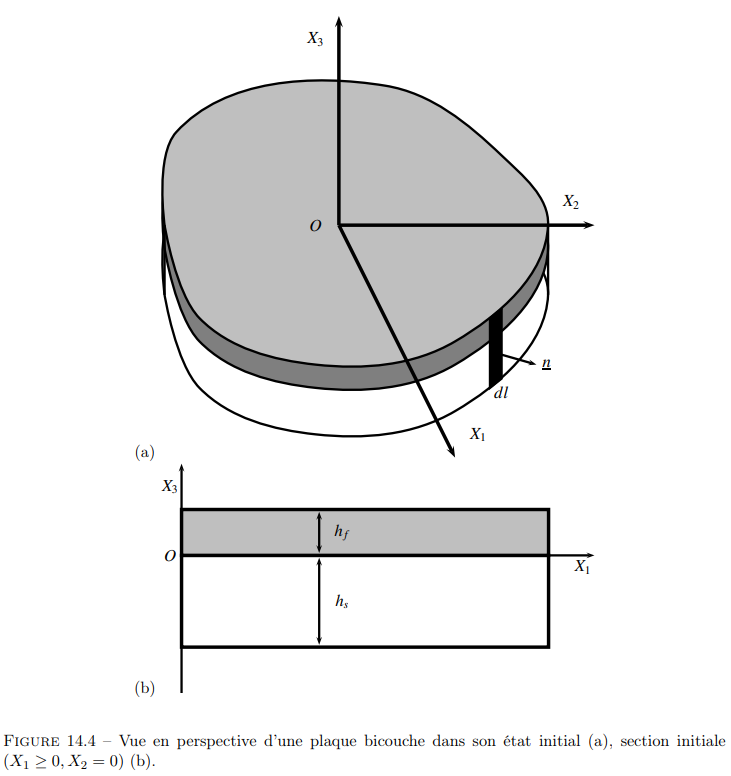
\includegraphics[scale=0.5]{imgs/surface_etude.png}
    \end{figure}
\end{frame}

\begin{frame}
    \frametitle{Torseur des efforts résultants}
    En notant $\partial S_l$ le contour de largeur $dl$, on a donc la résultante suivante des efforts surfaciques :
    $$\underline{R^{s}} = \int_{\partial S_l \times ]-h_s,h_f[}\underline{t}\;ds = \int_{\partial S_l \times ]-h_s,h_f[}\underset{\sim}{\sigma}\cdot\underline{n}\;dl\;dX_3$$
    On introduit la résultante linéique, en divisant par la largeur $dl$ :
    $$\underline{R} = \int_{-h_s}^{h_f}\underset{\sim}{\sigma}\cdot\underline{n}\;dX_3$$
    $n_3 = 0$ donc $R_3 = 0$. On calcule $R_1$ et $R_2$ :
    $$R_1 = \int_{-h_s}^{h_f}\sigma_{11}\;n_1\;dX_3 = (\int_{-h_s}^{h_f}\sigma_{11}\;dX_3)n_1$$
    $$R_2 = \int_{-h_s}^{h_f}\sigma_{22}\;n_2\;dX_3 = (\int_{-h_s}^{h_f}\sigma_{22}\;dX_3)n_2$$
\end{frame}

\begin{frame}
    \frametitle{Torseur des efforts résultants}
    On calcule aussi le moment résultant des efforts surfaciques, par rapport au point $O$ :
    $$\underline{M^{s}} = \int_{\partial S_l \times ]-h_s,h_f[}\underline{X}\wedge \underline{t}\;ds$$
    On introduit de même la résultante linéique, en divisant par la largeur $dl$ :
    $$\underline{M} = \int_{-h_s}^{h_f}\underline{X}\wedge (\underset{\sim}{\sigma}\cdot\underline{n})\;dX_3 = \int_{-h_s}^{h_f}\begin{pmatrix} X_1 \\ X_2 \\ X_3 \end{pmatrix}\wedge \begin{pmatrix} \sigma_{11}\;n_1 \\ \sigma_{22}\;n_2 \\ 0 \end{pmatrix}\;dX_3$$
    D'où $$\underline{M} = \int_{-h_s}^{h_f}\begin{pmatrix} -X_3\;\sigma_{22}\;n_2 \\ \sigma_{11}\;n_1\;X_3 \\ \sigma_{22}\;X_1\;n_2 - X_2\;\sigma_{11}\;n_1 \end{pmatrix}\;dX_3$$
\end{frame}

\begin{frame}
    \frametitle{Torseur des efforts résultants}
    Pour récapituler :
    $$R_1 = (\int_{-h_s}^{h_f}\sigma_{11}\;dX_3)n_1$$
    $$R_2 = (\int_{-h_s}^{h_f}\sigma_{22}\;dX_3)n_2$$
    $$M_1 = (\int_{-h_s}^{h_f} -X_3\;\sigma_{11}\;dX_3)n_2$$
    $$M_2 = (\int_{-h_s}^{h_f} X_3\;\sigma_{11}\;dX_3)n_1$$
    $$M_3 = (n_2\;X_1\;\int_{-h_s}^{h_f} \sigma_{11}\;dX_3 - n_1\;X_2 \int_{-h_s}^{h_f} \sigma_{11}\;dX_3$$
    Il suffit de calculer $\int_{-h_s}^{h_f}\sigma_{11}\;dX_3$ et $\int_{-h_s}^{h_f}X_3\;\sigma_{11}\;dX_3$ !
\end{frame}

\begin{frame}
    \frametitle{Torseur des efforts résultants}
    D'une part :
    $$\int_{-h_s}^{h_f}\sigma_{11}\;dX_3$$ $$=\int_{-h_s}^{0}M_s(AX_3+C-\alpha_s(T-T_0))\;dX_3+\int_{0}^{h_f}M_f(AX_3+C-\alpha_f(T-T_0))\;dX_3$$
    $$=-M_sA\frac{h_s^{2}}{2}+M_s(C-\alpha_s(T-T_0))h_s+M_fA\frac{h_f^{2}}{2}+M_f(C-\alpha_f(T-T_0))h_f$$
    D'autre part :
    $$\int_{-h_s}^{h_f}\sigma_{11}\;X_3\;dX_3$$
    $$=M_sA\frac{h_s^{3}}{3}-M_s(C-\alpha_s(T-T_0))\frac{h_s^{2}}{2}+M_fA\frac{h_f^{3}}{3}+M_f(C-\alpha_f(T-T_0))\frac{h_f^{2}}{2}$$
\end{frame}

\begin{frame}
    \frametitle{Torseur des efforts résultants}
    Par la loi fondamentale de la dynamique, les deux résultantes du torseur sont nulles.
    
    $\underline{n}$ étant non nul, les deux intégrales précédentes sont donc nulles.
    
    D'où le système :
    $$
    \left \{
    \begin{array}{rcl}
    (M_fh_f^{2}-M_sh_s^{2})\frac{A}{2}+(M_sh_s+M_fh_f)C&=&(M_sh_s\alpha_s+M_fh_f\alpha_f)(T-T_0) \\
    (Msh_s^{3}+M_fh_f^{3})\frac{A}{3}+(M_fh_f^{2}-M_sh_s^{2})\frac{C}{2}&=&(M_fh_f^{2}\alpha_f-M_sh_s^{2}\alpha_s)\frac{T-T_0}{2}
    \end{array}
    \right.
    $$
    \textbf{Principe de Saint-Venant} : solution satisfaisante loin du bord (valide presque partout si $\frac{h}{L}\ll1$)
\end{frame}

\subsection{Comparaison avec un modèle numérique}

\begin{frame}{Comparaison avec un modèle numérique}
    \begin{figure}
        \centering
        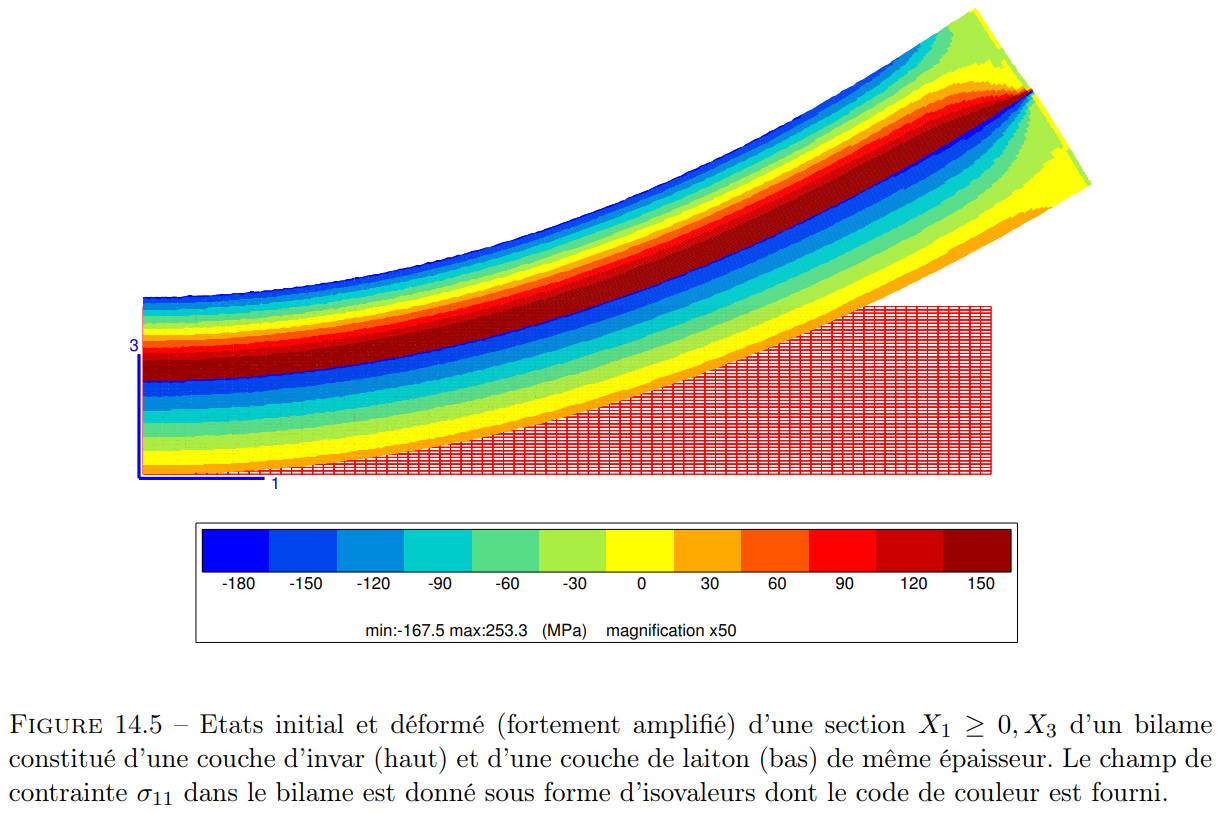
\includegraphics[scale=0.5]{imgs/simul_num.png}
    \end{figure}
\end{frame}

\subsection{Résolution du système}

\begin{frame}{Résolution du système}
    Le système précédent admet comme solution :
    $$A = 6\frac{M_fh_f}{M_sh_{s}^{2}}(\alpha_f-\alpha_s)(T-T_0)(1+\frac{h_f}{h_s})\Delta^{-1}$$
    $$\Delta = 1+4\frac{M_f}{M_s}\frac{h_f}{h_s}+6\frac{M_f}{M_s}\frac{h_f^2}{h_s^2}+4\frac{M_f}{M_s}\frac{h_f^3}{h_s^3}+\frac{M_f^2}{M_s^2}\frac{h_f^4}{h_s^4}$$
    $$C = (\alpha_s+4\alpha_f\frac{M_f}{M_s}\frac{h_f}{h_s}+3(\alpha_s+\alpha_f)\frac{M_f}{M_s}\frac{h_f^2}{h_s^2}+4\alpha_s\frac{M_f}{M_s}\frac{h_f^3}{h_s^3}+\alpha_f\frac{M_f^2}{M_s^2}\frac{h_f^4}{h_s^4})(T-T_0)\Delta^{-1}$$
\end{frame}

\subsection{Bilame de laiton et d'invar}

\begin{frame}{Application : bilame de laiton et d'invar}
    Utilisation de ce type de bilame : \textbf{cannes thermiques dans les chauffe-eau}
    \begin{figure}
        \centering
        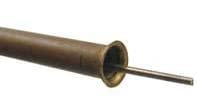
\includegraphics[scale=0.7]{imgs/canne_thermique.jpg}
        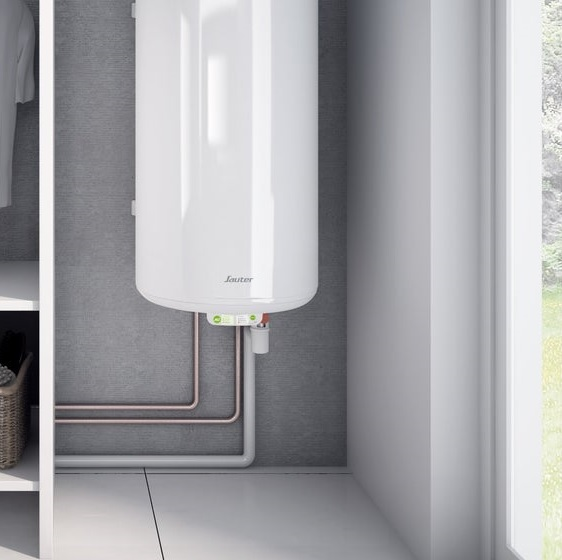
\includegraphics[scale=0.5]{imgs/chauffe_eau.jpg}
    \end{figure}
    
\end{frame}

\begin{frame}{Application : bilame de laiton et d'invar}
    \textbf{\Large{Validité du contexte infinitésimal}}
    
    Pour ce bilame laiton/invar, $h_s = h_f = \frac{h}{2}$ et $\frac{M_f}{M_s} = 2$, d'où :
    $$\Delta = 1+4\cdot2\cdot1+6\cdot2\cdot1+4\cdot2\cdot1+2^{2}\cdot1 = 33$$
    $$A = \frac{8}{11}(\alpha_f-\alpha_s)\frac{T-T_0}{h_s}$$
    $$C = \frac{T-T_0}{11}(5\alpha_s+6\alpha_f)$$
    
    On doit avoir $||Grad(\underline{u})|| \ll 1$.
    $$\frac{\partial u_1}{\partial X_1} = A X_3+C,\; \frac{\partial u_1}{\partial X_3} = A X_1,\; \frac{\partial u_3}{\partial X_1} = -A X_1$$
    $$\frac{\partial u_3}{\partial X_3} = -\frac{2\nu}{1-\nu}(A X_3 + C) + \frac{1+\nu}{1-\nu}\alpha(T-T_0)$$
\end{frame}

\begin{frame}{Application : bilame de laiton et d'invar}
    \textbf{Conditions suffisantes :}
    \begin{itemize}
        \item $|\alpha_s(T-T_0)|\ll 1 \rightarrow$ contrôle de $|A X_3|$ et $|C|$
        \item $|\alpha_f(T-T_0)|\ll 1 \rightarrow$ contrôle de $|A X_3|$ et $|C|$
        \item $|(\alpha_s-\alpha_f)(T-T_0)|\frac{L}{h_s}\ll 1 \rightarrow$ contrôle de $|A X_1|$
    \end{itemize}
    Pour le laiton/invar :
    \begin{itemize}
        \item $|\alpha_s(T-T_0)|\approx19\cdot10^{-6}\cdot100\ll1$
        \item $|\alpha_f(T-T_0)|\approx1.2\cdot10^{-6}\cdot100\ll1$
        \item $\frac{L}{h_s}\ll \frac{1}{|(\alpha_s-\alpha_f)(T-T_0)|} \approx \frac{1}{17.8\cdot 10^{-4}}\approx 5\cdot 10^{-6}$
    \end{itemize}
\end{frame}

\begin{frame}{Application : bilame de laiton et d'invar}
    \textbf{\Large{Profils de déplacement}}
    
    \begin{itemize}
        \item A l'interface, en $X_3=0$:
    \end{itemize}
    \begin{figure}
        \centering
        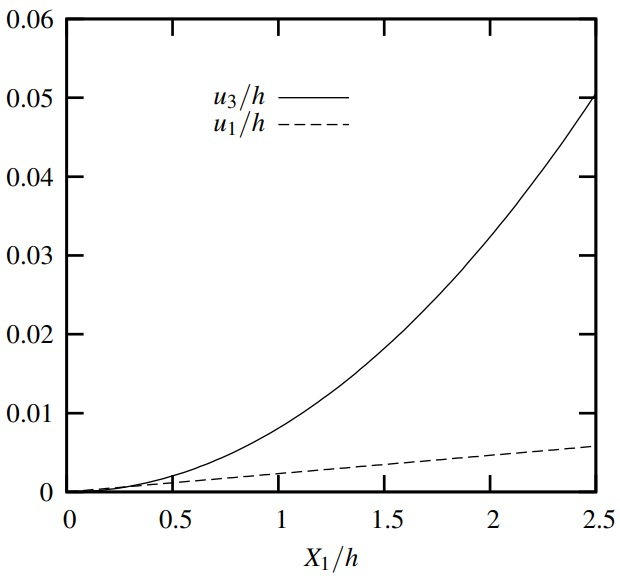
\includegraphics[scale=0.5]{imgs/graph1.jpg}
        \caption{Déplacements de l'interface du bicouche $X_3=0$}
    \end{figure}
\end{frame}

\begin{frame}{Application : bilame de laiton et d'invar}
    \textbf{\Large{Profils de déformation}}
    
    \begin{itemize}
        \item Sur l'axe $X_1=X_2=0$:
    \end{itemize}
    \begin{figure}
        \centering
        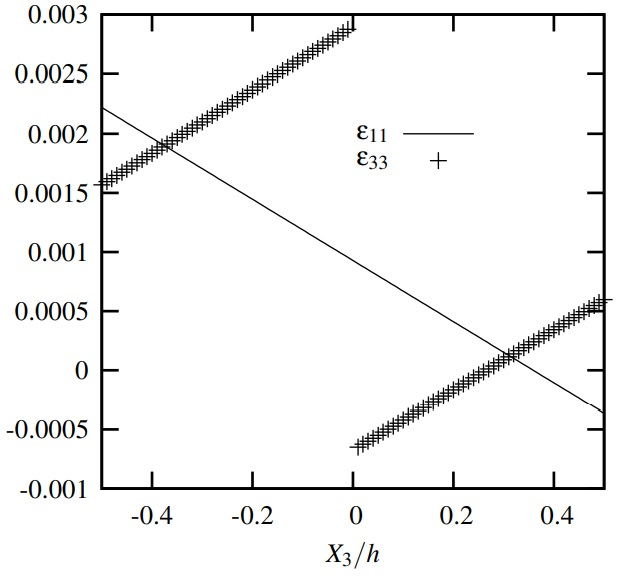
\includegraphics[scale=0.5]{imgs/graph2.jpg}
        \caption{Déformations le long de l'axe $X_1=X_2=0$}
    \end{figure}
\end{frame}

\begin{frame}{Application : bilame de laiton et d'invar}
    \textbf{\Large{Profils de contrainte}}
    
    \begin{itemize}
        \item Sur l'axe $X_1=X_2=0$:
    \end{itemize}
    \begin{figure}
        \centering
        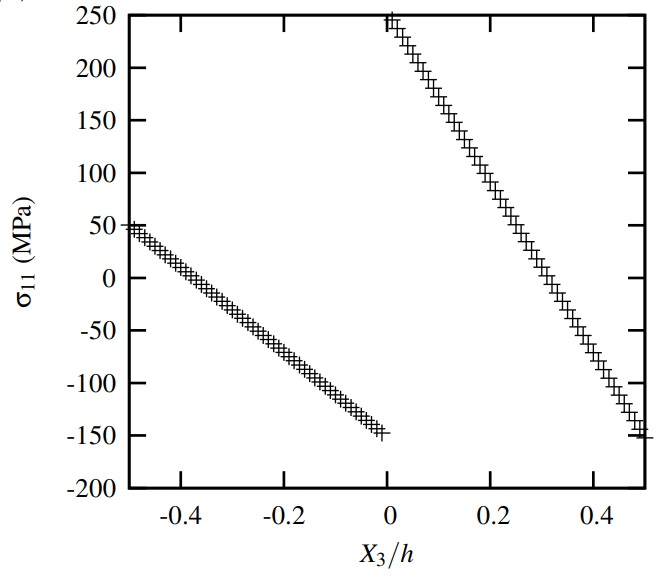
\includegraphics[scale=0.5]{imgs/graph3.jpg}
        \caption{Contraintes le long de l'axe $X_1=X_2=0$}
    \end{figure}
    Contrainte maximale atteinte pour $\frac{X_3}{h_s} = 0^+ : \sigma_{max} = 253 MPa$
\end{frame}